\documentclass[12pt]{scrartcl}
\usepackage{graphicx}

\begin{document}

\begin{titlepage}
\begin{center}

\vspace*{3.0 cm}
{\Huge Public Static Void Main}\\[0.7cm]
{\Large Requirements Document, Version 1}\\[3.8cm]
{\Large \today}\\[0.5cm]
Adam Schwalm\\
Eli Hunnicutt\\
Andrew LaFrance\\
Tyler Bertrand\\
Martin Kinsey\\[4.0cm]

Group Number: 5\\
Lab Instructor: Ajay Bandi
  

  
\end{center}
\end{titlepage}


\newpage\null\thispagestyle{empty}\newpage

\tableofcontents

\newpage\null\thispagestyle{empty}\newpage

\section{Introduction}
\subsection{Purpose}
The purpose of this Requirements Document is to specify the software requirements of the Public Static Void Main project, a programming forum that will allow users to create posts and images, as well as maintain user profiles. The document will help to define the concept and functionality of Public Static Void Main.
 
The intended audience of this document is the software developers, Mr. Bandi, and Mr. Anderson.
 
\subsection{Definitions, Acronyms, and Abbreviations}
\begin{description}
\item [PSVM]          	Acronym for “Public Static Void Main”
\item [User]            The standard visitor to PSVM. Can create/edit posts and maintain a user profile
\item [User Profile] 	A page specific to one user. Contains information about the user, their avatar, etc.
\item [Admin]         	A special class of user. Can delete posts and ban users
\item [Post]            A piece of original content, such as the beginning of a discussion, or an image
\item [Comment]			A comment upon a post
\item [Thread]			A page containing a post and all of its comments
\item [Subforum]  A mini forum dedicated to a single subject such as a specific programming languag
\end{description}
\section{System Overview}
\subsection{Purpose}

PSVM (Public Static Void Main) is a programming centric forum. Like most forums, the user will be able to create threads and posts as well as search the forum. Users will have profiles which will allow them to set signatures and change user settings.  The users will be able to message other users using a built-in “private messaging” feature. Administrators will be able to lock and delete threads as well as ban users.

\subsection{Use Case Diagram}

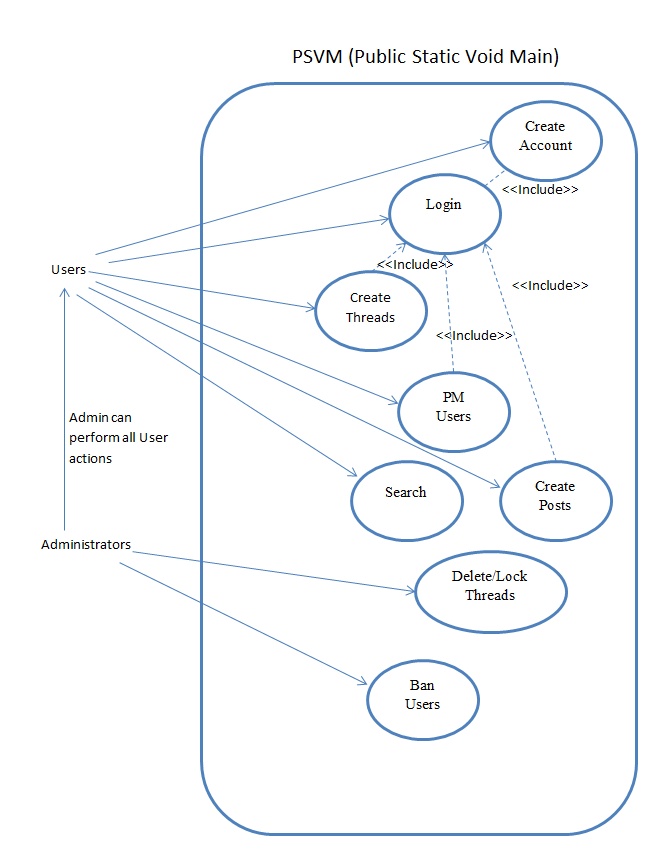
\includegraphics{use-case.PNG}

\section{Specific Requirements}
\subsection{Create Account (Required)}
\subsubsection{Description}

The user is required to be logged-in to perform various actions (make posts, edit profile, etc.).
In order to detect valid users, user account creation is required. 

\subsubsection{Actors}

Users

\subsubsection{Steps}

\begin{enumerate}
\item The user clicks the ``Register'' link at the top of the main page
\item User is prompted for a username and password (twice for verification)
\item A new account is created for the user in the database
\item The user is redirected to the main page and logged-in
\end{enumerate}

\subsection{Edit Posts (Required)}
\subsubsection{Description}

User changes the text of a comment or post they created within the forum

\subsubsection{Actors}

Users

\subsubsection{Steps}

\begin{enumerate}
\item User logs in
\item User starts at the thread page he commented on.
\item Page displays ‘edit’ button alongside posts this user made
\item User clicks on ‘edit’
\item Application opens the text editor, with the text of his post inside it.
\item User can change the text
\item User hits submit
\item  Application saves the changes, modifying the saved post
\end{enumerate}

\subsection{PM Other Users (Medium)}
\subsubsection{Description}

Most forums have a feature allowing users to message eachother through the site. This
feature allows such behaviour.

\subsubsection{Actors}

Users

\subsubsection{Steps}
\begin{enumerate}
\item User logs in
\item User selects the ``PM'' button from the main page or their user page.
\item The User types the username of the user to receive the message
\item User presses the ``Send'' button.
\end{enumerate}

\subsection{Quote Post (Required)}
\subsubsection{Description}

The user can select a previous post to quote in their post. When quoting a post, the quote is contained in unique html to distinguish from the standard post. 
\subsubsection{Actors}

Users

\subsubsection{Steps}

\begin{enumerate}
\item User logs in
\item The user clicks a button under a post called Quote
\item The quote then appears in the post box for the user to add more content
\item When the post is submitted, the quote displays in the post with the special quote html
\end{enumerate}

\subsection{Create Subforum (Required)}
\subsubsection{Description}
Subforums are sections of the forum containing threads that are alike. This allows admins to create a new subforum on the site. Subforum contain a title and a brief description of what to post in the subforum.

\subsubsection{Actors}

Admin

\subsubsection{Steps}
\begin {enumerate}
\item Admin logs in
\item Admin enters home page
\item Admin navigates to admin tools
\item Admin uses admin tools to create a new subforum
\item Application prompts user for a title and description for the subforum
\item Admin fills out form
\item Admin confirms completion
\item Application stores subforum information
\end {enumerate}


\subsection{Create Thread (Requried)}
\subsubsection{Description}

The user can create a new thread. The thread is a user title collection of posts that any user can post to. The original user has the first post in the thread.

\subsubsection{Actors}

Users

\subsubsection{Steps}

\begin{enumerate}
\item User logs in
\item The user clicks a button called Create Post 
\item The user enters the title of the new thread and the location of where to post the thread
\item The user enters the first post for the thread
\item The user presses the submit thread button
\item The thread is posted under the proper heading
\end{enumerate}

\subsection{Custom User Signatures (Medium)}
\subsubsection{Description}

Each user can customize a personal signature that will be placed below each post they make. This signature can be constructed from plain text.

\subsubsection{Actors}

Users

\subsubsection{Steps}

\begin{enumerate}
\item User logs in
\item The user clicks the link to go to their profile.
\item The user clicks the link to edit their profile.
\item The user clicks the link to edit their signature.
\item The user enters their desired signature in the text box provided.
\item The user clicks the button to save their signature.
\item The page redirects to the users profile page.
\item The signature appears under every post the user makes to any thread.
\end{enumerate}

\subsection{Delete Posts (Required)}
\subsubsection{Description}

Each user can navigate to any post they have made in any thread and permanently delete the post.

\subsubsection{Actors}

Users

\subsubsection{Steps}

\begin{enumerate}
\item User logs in
\item The user finds the thread containing the post they want to delete.
\item The user scrolls to the post that they want to delete.
\item The user clicks the link to delete the post.
\item The page asks the user to confirm the delete request.
\item The user confirms the request.
\item The post is deleted, and the thread pulls the posts below it up to fill the gap.
\end{enumerate}



\subsection{Report Users (Requried)}
\subsubsection{Description}

Each user can navigate to the offending user’s profile page and select “Report User”. The user then enters a reason for reporting the offending user (breaking rules, threats, etc.), and confirms the report user request.

\subsubsection{Actors}

Users

\subsubsection{Steps}

\begin{enumerate}
\item User logs in
\item The user navigates to the offending user’s profile page.
\item The user selects the “Report User” option from a list of options.
\item The page prompts the user to enter a reason for reporting the offending user.
\item The page asks the user to confirm the request.
\item The user confirms the request.
\item The post is deleted, and the thread pulls the posts below it up to fill the gap.
\end{enumerate}


\subsection{Change Password (Required)}
\subsubsection{Description}

The user may change their password from their user profile page by selecting “change password.” The user will be required to enter their original password as well as the new password.

\subsubsection{Actors}

Users

\subsubsection{Steps}

\begin{enumerate}
\item User logs in
\item The user clicks the button to navigate to to their profile page
\item The user clicks the “change password” button to navigate to the change password page
\item The user enters their current password
\item The user enters their new password
\item The user selects the “change password” button to confirm the password change
\end{enumerate}

\subsection{View User Profile (Required)}
\subsubsection{Description}

The user may view another user’s profile page by selecting the “view profile” button next to a post the user has made

\subsubsection{Actors}

Users

\subsubsection{Steps}

\begin{enumerate}
\item The user clicks the “view profile” button next to a post made by the user whose profile they wish to view
\item The user is navigated to the selected user’s profile page
\end{enumerate}

\subsection{Browse Posts (Required)}
\subsubsection{Description}
Each of the subforum pages has a listing of the posts and threads made within that subforum. Users can view the list, which contains
information about each post, such as the number of “likes” it has received, or the number of comments upon it.

\subsubsection {Actors}
User

\subsubsection{Steps}
\begin {enumerate}
\item User logs in
\item User navigates to the desired forum
\item Application presents the user with the most recent posts within that forum
\item User selects a post to view
\end{enumerate}

\subsection{Search Subforum (Requried)}
\subsubsection{Description}
The user can initiate a search within a subforum, at which point the application returns a list of the posts with relevant titles and tags.

\subsubsection{Actors}
User

\subsubsection{Steps}
\begin{enumerate}
\item User logs in
\item User navigates to desired subforum
\item User enters the search terms into the search box
\item Application reviews database for posts matching the search terms
\item Application returns best results
\item User selects desired returned post
\end {enumerate}

\subsection{“Like” Posts (Medium)}
\subsubsection{Description}
Within a post’s thread, a button is located next to or below the post’s content. Pressing this button adds a “like” to the post’s count, which is used to
determine which posts show up on the front page of the forum, as well as being a general gauge of the content’s popularity.

\subsubsection{Actors}
Users
\subsubsection{Steps}

\begin{enumerate}
\item The user logs into the website
\item The user presses the like button under a current post
\item Like appears under the post 
\end{enumerate}


\subsection{Upload User Image (Medium)}
\subsubsection{Description}

Users can upload an image to their profile which will be displayed next to their posts, or by PMs they send to other users.

\subsubsection{Actors}

Users

\subsubsection{Steps}
\begin{enumerate}
\item User logins into the system
\item Navigate to the profile page
\item User clicks the ``Upload profile picture'' button
\item Selects an image to upload
\item The image is uploaded to the server and displayed next to the users name
\end{enumerate}



\subsection{Tag Threads (Medium)}
\subsubsection{Description}

Threads may be ``tagged'' with labels indicating their content. This can help identify the keywords for the search engine, or other interested users.

\subsubsection{Actors}

Users

\subsubsection{Steps}
\begin{enumerate}
\item User logs in
\item User creates a thread
\item While creating the thread, the user lists ``tags''
\item Other users will be presented with this thread when searching
\end{enumerate}


\subsection{Embeded HTML (Medium)}
\subsubsection{Description}

It can sometimes be useful to embed limited HTML in a post (i.e., for hotlinking images or embeding youtube videos).

\subsubsection{Actors}

Users

\subsubsection{Steps}
\begin{enumerate}
\item User logs in
\item User creates a post
\item While writting the post, the users uses a 'markup' language to format code/make link, etc.
\item When the user submits the post, the server adds the html formatting
\end{enumerate}

\subsection{Pin Thread (Required)}
\subsubsection{Description}
Admins can pin a thread to the top of a category. This post will always appear at top of the page.
This function will be used by admin if the post is important and needs to be seen by all users.

\subsubsection{Actors}

Admin

\subsubsection{Steps}

\begin{enumerate}
\item The admin logs in
\item The admin navigates to the category of the thread
\item The admin press the pin button next to the title of the thread
\end{enumerate}

\subsection{Edit Signature (Medium)}
\subsubsection{Description}
Allows the user to change their signature, a line that appears under any comment they make. By default, there is no signature.

\subsubsection{Actors}
User

\subsubsection{Steps}
\begin {enumerate}
\item User logs in
\item User navigates to their profile page
\item User selects the “Edit Signature” option next to the signature display box
\item The application presents the user with a text box
\item User fills out text form with the desired signature
\item User confirms completion
\item Application stores the changed signature in the database
\end {enumerate}

\subsection{Edit Description (Requried)}
\subsubsection{Description}
Allows the user to change the description within their profile.
The description field is used to share information about themselves, their posting habits, or their coding abilities/expertise.

\subsubsection {Actors}
User

\subsubsection {Steps}
\begin {enumerate}
\item The User logs in
\item User navigates to their profile page
\item User selects the “Edit Description” option next to the description field
\item Application presents user with a text form to enter the desired description
\item User fills out the text form with the description
\item User confirms completion
\item Application stores the changed description in the database
\end {enumerate}


\subsection{Move Thread (Required)}
\subsubsection{Description}
Admins can move a thread to a different category.
If the thread posted by a user is better fitted for another category the admins can move the thread into the better category. 

\subsubsection{Actors}

Admin

\subsubsection{Steps}
\begin {enumerate}
\item Admin logs in
\item Admin browses to the thread that needs to be moved
\item Admin selects the “move” option
\item System prompts the admin for the forum to move thread to
\item Admin confirms
\item System moves thread
\end {enumerate}



\subsection{Ban Users (Required)}
\subsubsection{Description}
 
Admin removes a user’s access to the forum

\subsubsection{Actors}
 
Admin
 
\subsubsection{Steps}
\begin{enumerate}
\item Admin logs in
\item Admin begins on the profile page of the user he intends to ban
\item Application displays a list of commands at the top of the page, among which is ‘ban’
\item Admin selects the ban command
\item Application prompts to confirm the ban request
\item Admin confirms
\item Application removes the user from the user list, adds the username to a blacklist
\item Application displays a confirmation of the user’s removal
\end {enumerate}



\subsection{Lock Thread (Required)}
\subsubsection{Description}
Admins can lock a thread, so no more posts can be made to the thread. Threads can be lock only by Admins.
If a thread is going off-topic or against the rules of the site, the thread can be closed 

\subsubsection{Actors}

Admin
\subsubsection{Steps}

\begin{enumerate}
\item The admin logs into the webpage
\item The admin browses to the category of the thread 
\item The admin presses the button of a lock next to the thread title
\end{enumerate}


\subsection{Edit Profile (Required)}
\subsubsection{Description}
The user can edit elements of their profile by clicking edit profile when viewing their own profile page.

\subsubsection{Actors}
User

\subsubsection{Steps}
\begin {enumerate}
\item User logs in to website
\item User navigates to their profile page
\item User can select the “Edit …” option next to any of their profile components (picture, description, or signature)
\item Application allows user to edit the item
\end {enumerate}


\subsection{Create Category (Medium)}
\subsubsection{Description}
Categories are sections of the forum containing threads that are alike.
This allows admins to create a new category on the site. Categories contain a title and a brief description of what to post in the category.






\subsection{Appendix A: User Interface}

\subsubsection{Root Page}

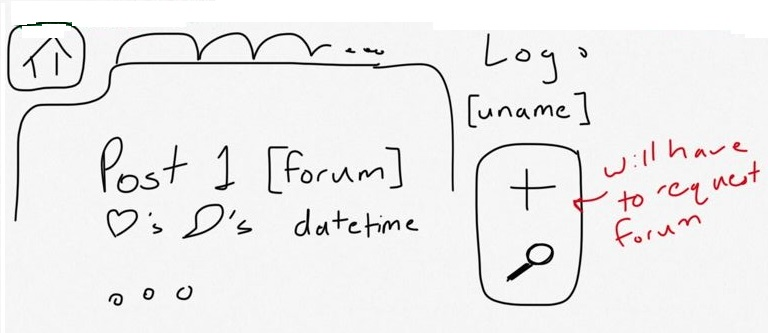
\includegraphics[width=17cm, height=17cm, keepaspectratio]{homepage.jpg}

The homepage, viewed upon entering the forum. Shows the “hottest” threads from various subforums.

\subsubsection{Forum Page}

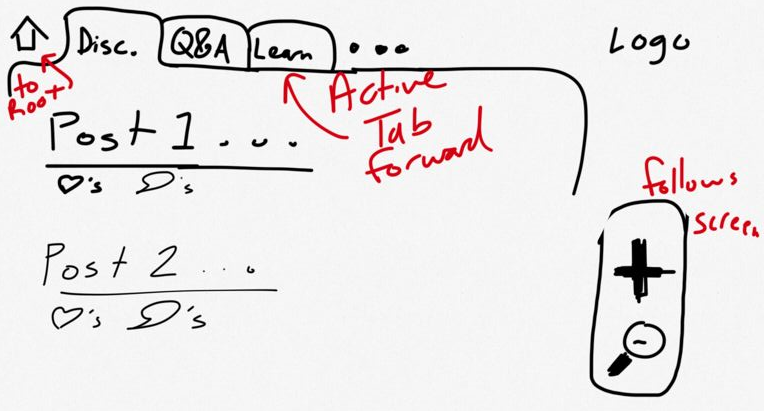
\includegraphics[width=17cm, height=17cm, keepaspectratio]{forumpage.png}

The home page for a specific subforum. Shows the newest posts within it, as well as information about them, such as “likes” and comments. The toolbar on the side follows the screen as the user scrolls up or down, and displays buttons for creating a new post, or searching for an existing post.

\subsubsection{Post Page}

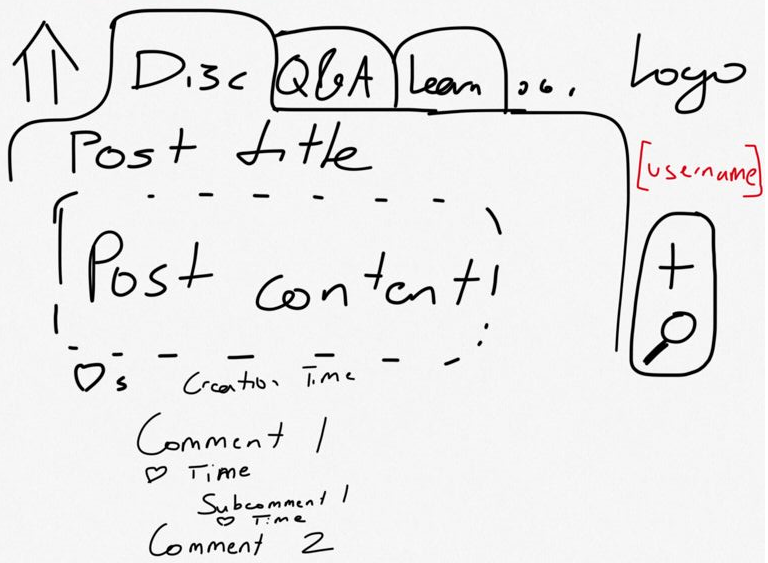
\includegraphics[width=17cm, height=17cm, keepaspectratio]{postpage.png}

The page for a specific post. Shows the post as well as information about it, all of the relevant comments, and information about them.

\subsubsection{Profile Page}

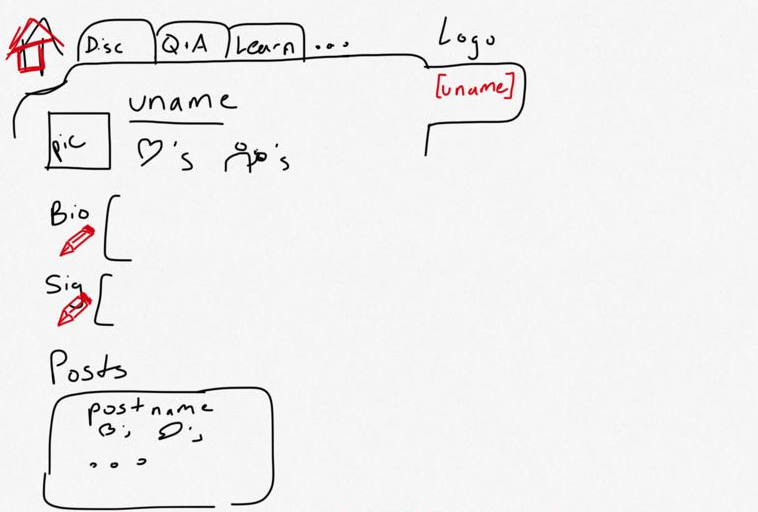
\includegraphics[width=17cm, height=17cm, keepaspectratio]{profilepage.png}

The page for a specific user’s profile. Displays the user’s name, profile picture / avatar, the total of their “likes” and friends, as well as their “bio” and their signature. Beneath those is the user’s history, showing some of their most recent posts.

p\subsection{Appendix B: Initial tasks and assignments}
\begin{description}
\item [Requirements Presentation] - Martin Kinsey
\item [Design Presentation] - Adam Schwalm, Andrew LaFrance
\item [Final Presentation] - Tyler Bertrand, Eli Hunnicutt
\vspace{4mm}
\item [Adam Schwalm] - Backend Design, Server work
\item [Eli Hunnicutt] - Javascript Management, Design
\item [Andrew LaFrance, Martin Kinsey] - Graphic Design, Frontend Design work
\item [Tyler Bertrand] - Database Design, Management
\end{description}
\end{document}

